\section{Implementation of the experiments}


In our program, many options are parametrizable. Those can be set using program arguments :
\begin{itemize}
\item The graph to play on (graphviz format supported)
\item The number of colors to play with
\item The number of games to play
\item The number of simulations to be run by Monte-Carlo before selecting a move
\end{itemize}
After some testing, we settled on the following experimental conditions :
\begin{itemize}
\item A number of simulations of 1000. This seemed to be a good compromize between speed and AI accuracy.
\item A number of games played of 1000. It seemed again to be a good compromize between computation time and statistical confidence. However, we could not play as much games on the 5x5 grids with a high number of colors (typically 4 or 5). We then tuned down the games to 100 for those cases. 
\end{itemize}

Here are the results :\\

\subsection{Chains}

\subsubsection{Odd number of vertices}

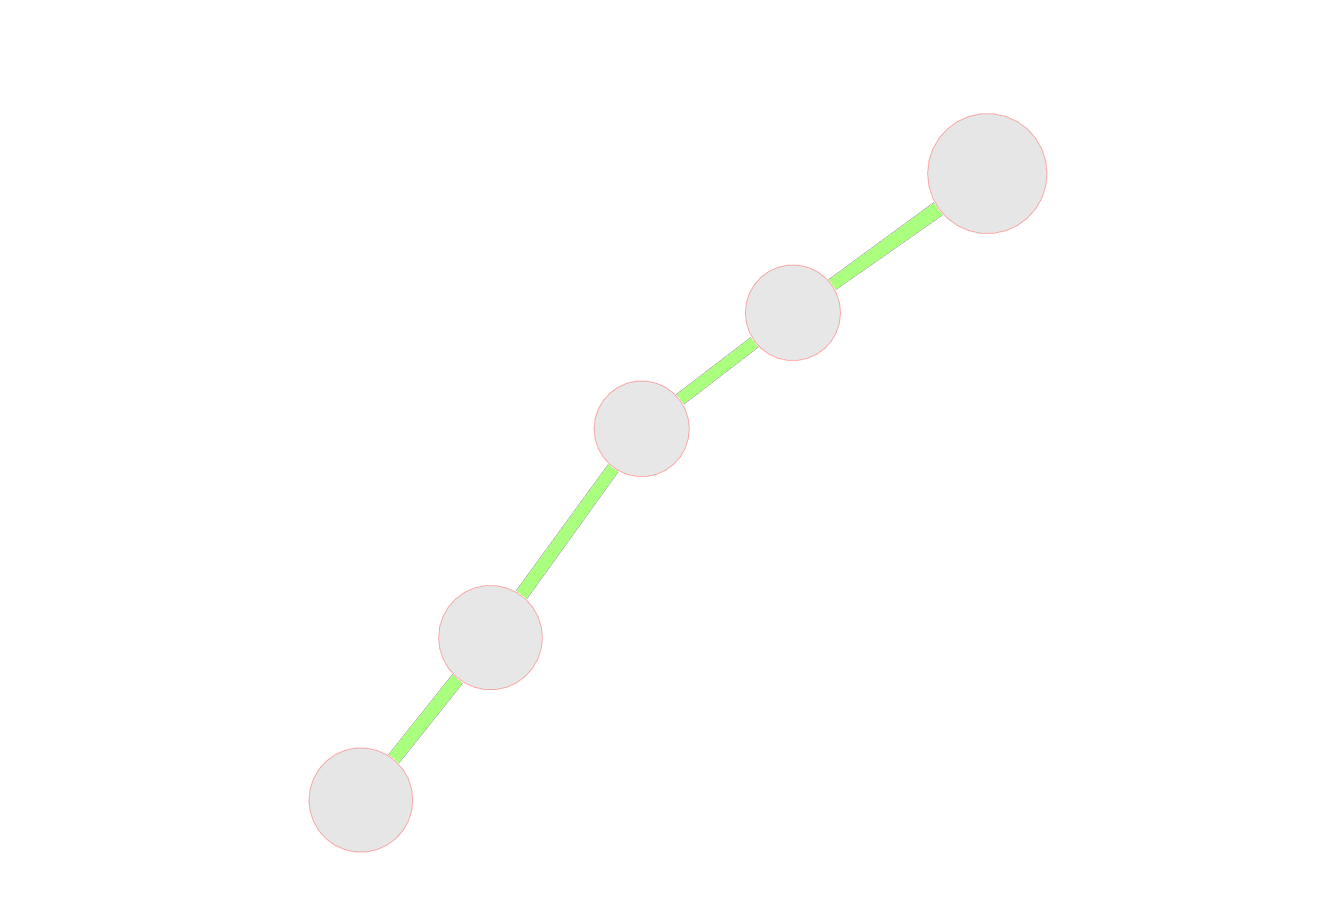
\includegraphics[width=11cm]{graphchaineimpaire.png}

\subsubsection{Even number of vertices}

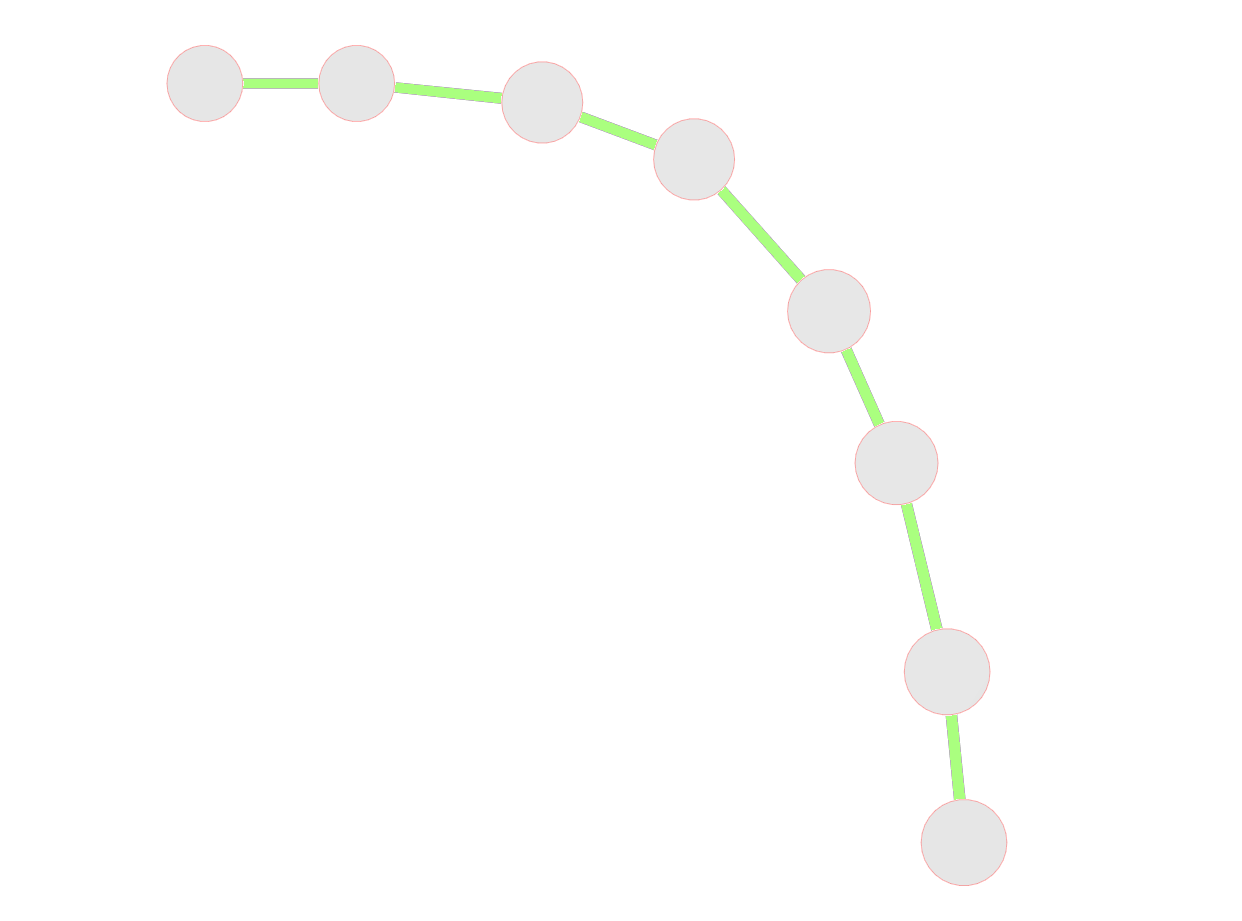
\includegraphics[width=11cm]{graphchainepaire.png}

\subsection{Cycles}

\subsubsection{Odd number of vertices}

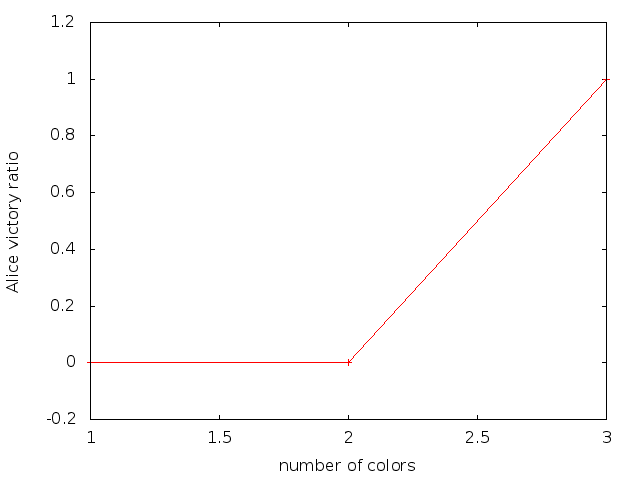
\includegraphics[width=11cm]{resultats/cycleimpair.png}

\subsubsection{Even number of vertices}

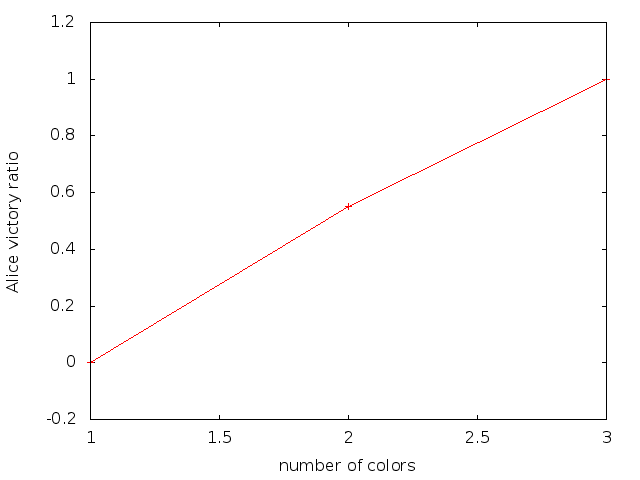
\includegraphics[width=11cm]{resultats/cyclepair.png}

\subsection{Grids}

\subsubsection{2x5}

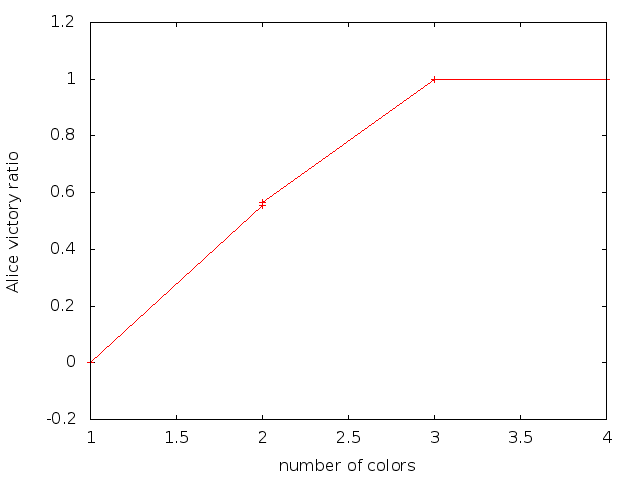
\includegraphics[width=11cm]{resultats/grille25.png}

\subsubsection{5x5}

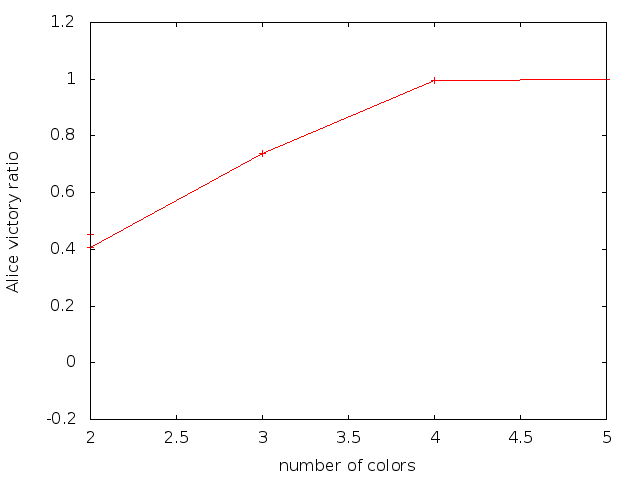
\includegraphics[width=11cm]{resultats/grille55.png}

\subsubsection{5x5 toroidal}

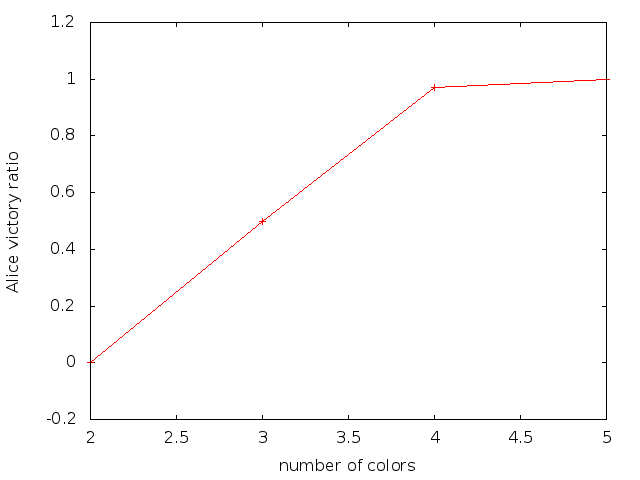
\includegraphics[width=11cm]{resultats/grilletor55.png}

\subsection{Binary Tree}

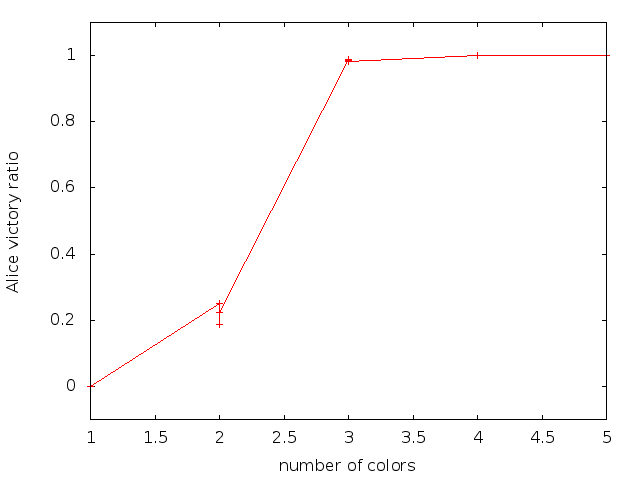
\includegraphics[width=11cm]{resultats/bintree3h.png}

\subsection{Non-Planar Graphs}

\subsubsection{Petersen Graph}

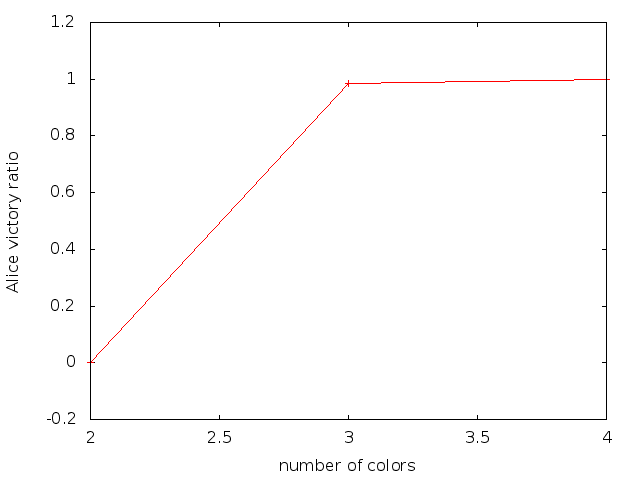
\includegraphics[width=11cm]{resultats/petersen.png}

\subsubsection{Icosaedron Graph}

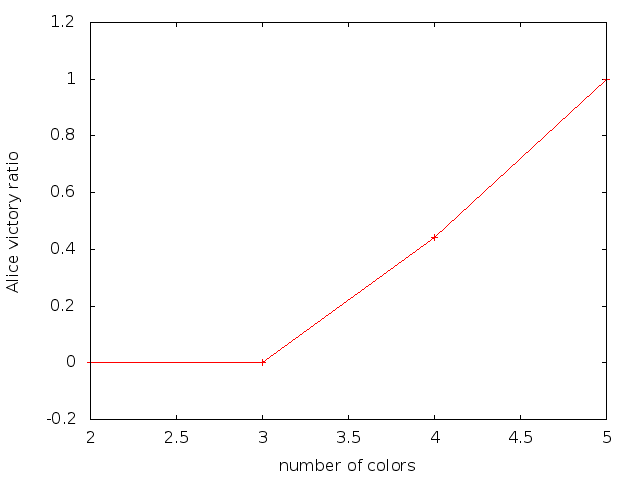
\includegraphics[width=11cm]{resultats/icosaedre.png}